\documentclass[xcolor={dvipsnames}]{beamer}
%\usepackage[utf8]{inputenc}
%\usetheme{Madrid}
%\usetheme{CambridgeUS}
\usetheme{Malmoe}
%\usecolortheme{beaver}
\usecolortheme{seahorse}

%-------------------------------------------------------------------------------
%          -Packages nécessaires pour écrire en Français et en UTF8-
%-------------------------------------------------------------------------------
\usepackage[utf8]{inputenc}
\usepackage[frenchb]{babel}
\usepackage[T1]{fontenc}
\usepackage{lmodern}
\usepackage{textcomp}

%-------------------------------------------------------------------------------

%-------------------------------------------------------------------------------
%                          -Outils de mise en forme-
%-------------------------------------------------------------------------------
\usepackage{hyperref}
\hypersetup{pdfstartview=XYZ}
\usepackage{enumerate}
\usepackage{graphicx}
%\usepackage{multicol}
%\usepackage{tabularx}

%\usepackage{anysize} %%pour pouvoir mettre les marges qu'on veut
%\marginsize{2.5cm}{2.5cm}{2.5cm}{2.5cm}

\usepackage{indentfirst} %%pour que les premier paragraphes soient aussi indentés
\usepackage{verbatim}
%\usepackage[table]{xcolor}  
%\usepackage{multirow}
\usepackage{ulem}
%-------------------------------------------------------------------------------


%-------------------------------------------------------------------------------
%                  -Nécessaires pour écrire des mathématiques-
%-------------------------------------------------------------------------------
\usepackage{amsfonts}
\usepackage{amssymb}
\usepackage{amsmath}
\usepackage{amsthm}
\usepackage{tikz}
\usepackage{xlop}
\usepackage[output-decimal-marker={,}]{siunitx}
%-------------------------------------------------------------------------------


%-------------------------------------------------------------------------------
%                    - Mise en forme 
%-------------------------------------------------------------------------------

\newcommand{\bu}[1]{\underline{\textbf{#1}}}


\usepackage{ifthen}


\newcommand{\ifTrue}[2]{\ifthenelse{\equal{#1}{true}}{#2}{$\qquad \qquad$}}

\newcommand{\kword}[1]{\textcolor{red}{\underline{#1}}}


%-------------------------------------------------------------------------------



%-------------------------------------------------------------------------------
%                    - Racourcis d'écriture -
%-------------------------------------------------------------------------------

% Angles orientés (couples de vecteurs)
\newcommand{\aopp}[2]{(\vec{#1}, \vec{#2})} %Les deuc vecteurs sont positifs
\newcommand{\aopn}[2]{(\vec{#1}, -\vec{#2})} %Le second vecteur est négatif
\newcommand{\aonp}[2]{(-\vec{#1}, \vec{#2})} %Le premier vecteur est négatif
\newcommand{\aonn}[2]{(-\vec{#1}, -\vec{#2})} %Les deux vecteurs sont négatifs

%Ensembles mathématiques
\newcommand{\naturels}{\mathbb{N}} %Nombres naturels
\newcommand{\relatifs}{\mathbb{Z}} %Nombres relatifs
\newcommand{\rationnels}{\mathbb{Q}} %Nombres rationnels
\newcommand{\reels}{\mathbb{R}} %Nombres réels
\newcommand{\complexes}{\mathbb{C}} %Nombres complexes


%Intégration des parenthèses aux cosinus
\newcommand{\cosP}[1]{\cos\left(#1\right)}
\newcommand{\sinP}[1]{\sin\left(#1\right)}

%Fractions
\newcommand{\myfrac}[2]{{\LARGE $\frac{#1}{#2}$}}

%Vocabulaire courrant
\newcommand{\cad}{c'est-à-dire}

%Droites
\newcommand{\dte}[1]{droite $(#1)$}
\newcommand{\fig}[1]{figure $#1$}
\newcommand{\sym}{symétrique}
\newcommand{\syms}{symétriques}
\newcommand{\asym}{axe de symétrie}
\newcommand{\asyms}{axes de symétrie}
\newcommand{\seg}[1]{$[#1]$}
\newcommand{\monAngle}[1]{$\widehat{#1}$}
\newcommand{\bissec}{bissectrice}
\newcommand{\mediat}{médiatrice}
\newcommand{\ddte}[1]{$[#1)$}

%Figures
\newcommand{\para}{parallélogramme}
\newcommand{\paras}{parallélogrammes}
\newcommand{\myquad}{quadrilatère}
\newcommand{\myquads}{quadrilatères}
\newcommand{\co}{côtés opposés}
\newcommand{\diag}{diagonale}
\newcommand{\diags}{diagonales}
\newcommand{\supp}{supplémentaires}
\newcommand{\car}{carré}
\newcommand{\cars}{carrés}
\newcommand{\rect}{rectangle}
\newcommand{\rects}{rectangles}
\newcommand{\los}{losange}
\newcommand{\loss}{losanges}


%----------------------------------------------------


\usepackage{../../../../pas-math}
\usepackage{../../../../moncours_beamer}

\usepackage{amssymb,amsmath}


\newcommand{\myitem}{\item[\textbullet]}

\graphicspath{{../img/}}

\title{Séquence 9 : Angles et parallélisme}
\subtitle{Correction des exercices}
%\author{O. FINOT}\institute{Collège S$^t$ Bernard}

%
%\AtBeginSection[]
%{
%	\begin{frame}
%		\frametitle{}
%		\tableofcontents[currentsection, hideallsubsections]
%	\end{frame} 
%
%}
%
%
%\AtBeginSubsection[]
%{
%	\begin{frame}
%		\frametitle{Sommaire}
%		\tableofcontents[currentsection, currentsubsection]
%	\end{frame} 
%}

\begin{document}



%\begin{frame}
%  \titlepage 
%\end{frame}


	

\begin{frame}
	\frametitle{Exercice 16}
	\begin{columns}
		\begin{column}{0.4\textwidth}
			\begin{center}
				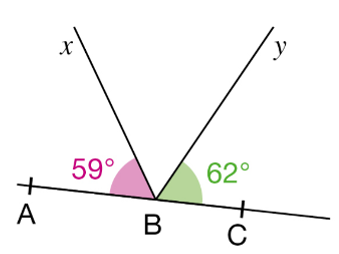
\includegraphics[scale=0.5]{16}\pause
			\end{center}
		\end{column}
		\begin{column}{0.6\textwidth}
			\begin{enumerate}
				\item Les points $A$, $B$ et $C$ sont alignés donc l'angle $\widehat{ABC}$ mesure 180\degree . 
				
				\begin{align*}
				\widehat{xBy} &= \widehat{ABC} - (\widehat{ABx}+ \widehat{yBC}) \\
				\widehat{xBy} &= 180 \degree - (59 \degree + 62 \degree) \\
				\widehat{xBy} &= 59\degree 
				\end{align*}\pause
				\item Les angles $\widehat{ABx}$ et $\widehat{xBy}$ ont la même mesure, donc la demi-droite $[Bx)$ est la bissectrice de l'angle $\widehat{ABy} $.
				%		\item 
			\end{enumerate}
		\end{column}
	\end{columns}
	
	
	
	
	
\end{frame}

\begin{frame}
	\frametitle{Exercice 17}
	
	\begin{columns}
		\begin{column}{0.4\textwidth}
			\begin{center}
				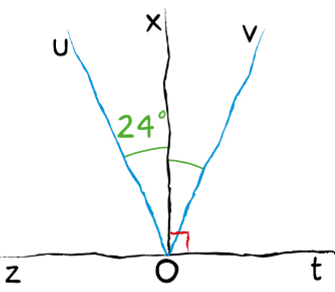
\includegraphics[scale=0.5]{17}\pause
			\end{center}
		\end{column}
		\begin{column}{0.6\textwidth}
			D'après le codage, les angles $\widehat{uOx}$ et $\widehat{xOv}$ ont la même mesure. \pause
			
			\begin{align*}
				\widehat{zOv} &= \widehat{zOx} + \widehat{xOv} \\
				\widehat{zOv} &= 90\degree + 24\degree \\
				\widehat{zOv} &= 104\degree
			\end{align*}
			
			L'angle $\widehat{zOv}$ mesure 104\degree.\pause
			
			De la même manière, l'angle $\widehat{tOu}$ mesure 104\degree.
		\end{column}
	\end{columns}
	
	
	
\end{frame}



\begin{frame}
	\frametitle{Exercice 18}
	
	\begin{columns}
		\begin{column}{0.4\textwidth}
			\begin{center}
				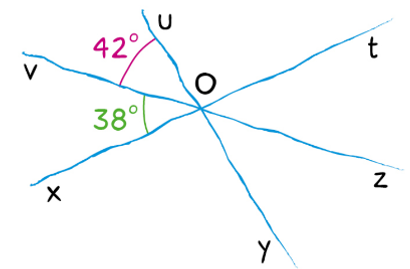
\includegraphics[scale=0.5]{18}\pause
			\end{center}
		\end{column}
		\begin{column}{0.6\textwidth}
			\begin{enumerate}[a.]
				\item L'angle opposé par le sommet à l'angle $\widehat{xOv}$ est l'angle $\widehat{tOz}$ \pause , il mesure 38\degree. \pause
				\item L'angle opposé par le sommet à l'angle $\widehat{xOz}$ est l'angle $\widehat{tOv}$ \pause , il mesure 142\degree. \pause
				\item L'angle opposé par le sommet à l'angle $\widehat{uOz}$ est l'angle $\widehat{yOv}$ \pause , il mesure 138\degree. \pause\\
				\item L'angle opposé par le sommet à l'angle $\widehat{tOu}$ est l'angle $\widehat{xOy}$ \pause , il mesure 100\degree. \pause
			\end{enumerate}
		\end{column}
	\end{columns}
	
	
	
\end{frame}


\begin{frame}
	\frametitle{Exercice 19}
	
	\begin{columns}
		\begin{column}{0.4\textwidth}
			\begin{center}
				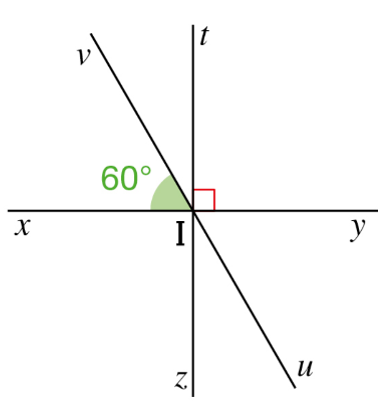
\includegraphics[scale=0.5]{19}\pause
			\end{center}
		\end{column}
		\begin{column}{0.6\textwidth}
			\begin{enumerate}[a.]
				\item L'angle  $\widehat{vIt}$ mesure 30\degree (90\degree - 60\degree) \pause
				\item L'angle  $\widehat{xIz}$ mesure 90\degree . \pause
				\item L'angle  $\widehat{zIu}$ est opposé par le sommet à l'angle $\widehat{vIt}$ il mesure 30\degree  \pause
				\item L'angle  $\widehat{uIy}$ est opposé par le sommet à l'angle $\widehat{xIv}$ il mesure 60\degree.
				
			\end{enumerate}
		\end{column}
	\end{columns}
	
	
	
\end{frame}
\end{document}